% Traceability: manual-local atomic field chapter.
\subsection{Atomic systems}

\subsubsection{Hydrogen shell scale witness}
\label{man:hydrogen-shell-scale-witness}
\colabbadge{manual/notebooks/04c_atomic_hydrogen_shells.ipynb}

\begin{table}[H]
\centering
\caption{Hydrogen retained-extraction declaration.}
\label{tab:hydrogen-retention}
\begin{threeparttable}
\begin{tabularx}{\linewidth}{@{}lX@{}}
\toprule
Item & Declaration \\
\midrule
Parent field & declared atomic AO field \\
Retained extraction & hydrogen shell field \\
Omitted context & non-hydrogen atomic contexts \\
First refinement & higher shell / local shell-report refinement \\
Validity window & declared shell record \\
Residual witness & pending until refinement row is computed \\
\bottomrule
\end{tabularx}
\end{threeparttable}
\end{table}

A declared hydrogen shell record is fixed first. Familiar hydrogen radii are attached afterward as a local shell report on the same shell record \cite{aod43_main_2026}.

\begin{table}[H]
\centering
\caption{Hydrogen shell declared row.}
\label{tab:hydrogen-shell-row}
\begin{threeparttable}
\small
\begin{tabularx}{\linewidth}{@{}lccccc@{}}
\toprule
Row & Shell band & $B^*$ & $\Lambda_b$ & $R_{\mathrm{loss}}$ [\(\mathrm{trit}/\mathrm{bip}_0\)] & Cadence witness \\
\midrule
H1 & 3 & 137 & 6 & $(1+8\ell_2)/24$ & $5/12$ \\
\bottomrule
\end{tabularx}
\ManualTableNote{The shell report remains local to this chapter. The declared row follows the shell-band, support, attenuation, and loss-channel machinery of the main note.}
\end{threeparttable}
\end{table}

\begin{table}[H]
\centering
\caption{Hydrogen shell radii comparison attached after the declared shell record.}
\label{tab:hydrogen-shell-radii}
\begin{threeparttable}
\small
\begin{tabularx}{\linewidth}{@{}llcccc@{}}
\toprule
Map & Subfamily & Calculated radius [m] & Declared benchmark [m] & Abs. error [m] & Rel. error [\%] \\
\midrule
\(\Phi_{\mathrm{shell}}\) & $n=1$ & $5.291772191461861\times10^{-11}$ & $5.291772109\times10^{-11}$ & $8.2461861\times10^{-19}$ & $1.5583\times10^{-6}$ \\
\(\Phi_{\mathrm{shell}}\) & $n=2$ & $2.1167088765847444\times10^{-10}$ & $2.1167088436\times10^{-10}$ & $3.29847444\times10^{-18}$ & $1.5583\times10^{-6}$ \\
\(\Phi_{\mathrm{shell}}\) & $n=3$ & $4.762594972315675\times10^{-10}$ & $4.7625948981\times10^{-10}$ & $7.4215675\times10^{-18}$ & $1.5583\times10^{-6}$ \\
\(\Phi_{\mathrm{shell}}\) & $n=4$ & $8.466835506338978\times10^{-10}$ & $8.4668353744\times10^{-10}$ & $1.31938978\times10^{-17}$ & $1.5583\times10^{-6}$ \\
\bottomrule
\end{tabularx}
\ManualTableNote{The calculated and reference radii are shown only after the declared shell record is fixed. Measurement-facing SI length renderings use the declared SI/constant layer~\cite{bipm_si_brochure_2025,nist_constants_complete}.}
\end{threeparttable}
\end{table}

\begin{figure}[H]
\centering
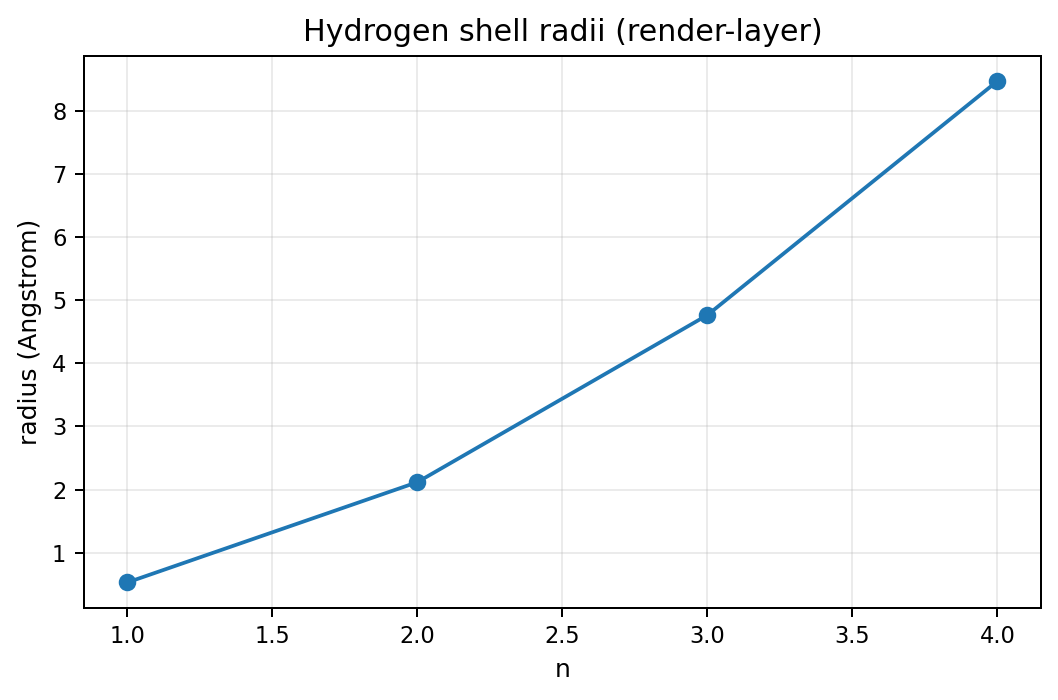
\includegraphics[width=0.74\linewidth]{figures/hydrogen/01_shell_radii.png}
\caption{Hydrogen shell radii witness.}
\label{fig:hydrogen-shell-radii}
\end{figure}

The declared hydrogen shell record carries the shell-band and attenuation witnesses of the main note, and the radii report is attached afterward as a local shell report.

\subsubsection{Nucleus confinement and neutron stability}
\label{man:nucleus-confinement-witness}
\colabbadge{manual/notebooks/04c_atomic_confinement.ipynb}

\begin{table}[H]
\centering
\caption{Confinement retained-extraction declaration.}
\label{tab:confinement-retention}
\begin{threeparttable}
\begin{tabularx}{\linewidth}{@{}lX@{}}
\toprule
Item & Declaration \\
\midrule
Parent field & declared atomic/nuclear AO field \\
Retained extraction & short-window confinement field \\
Omitted context & non-local nuclear contexts \\
First refinement & next shell/proximity refinement \\
Validity window & declared short window \\
Residual witness & qualitative until refinement row is computed \\
\bottomrule
\end{tabularx}
\end{threeparttable}
\end{table}

A short-window confinement class is fixed first and the same declared row reports proximity, confinement, and transmutation status.

\begin{table}[H]
\centering
\caption{Nucleus confinement declared rows.}
\label{tab:nucleus-confinement-row}
\begin{threeparttable}
\small
\begin{tabularx}{\linewidth}{@{}lXcclll@{}}
\toprule
Row & Structural key & $B^*$ & $\Lambda_b$ & Proximity & Confinement & Transmutation \\
\midrule
N1 & \texttt{tetron:3:3:6}, $(\lambda=3/2,137,\rho_2,V_4)$ & 137 & 6 & close & confined & 0 \\
N2 & \texttt{tetron:3:3:6}, $(\lambda=3/2,139,\rho_3,V_4)$ & 139 & 3 & failed & unconfined & 1 \\
\bottomrule
\end{tabularx}
\ManualTableNote{The same declared short row resolves shell signature, dominant rung, proximity, confinement, and transmutation status.}
\end{threeparttable}
\end{table}

\begin{figure}[H]
\centering
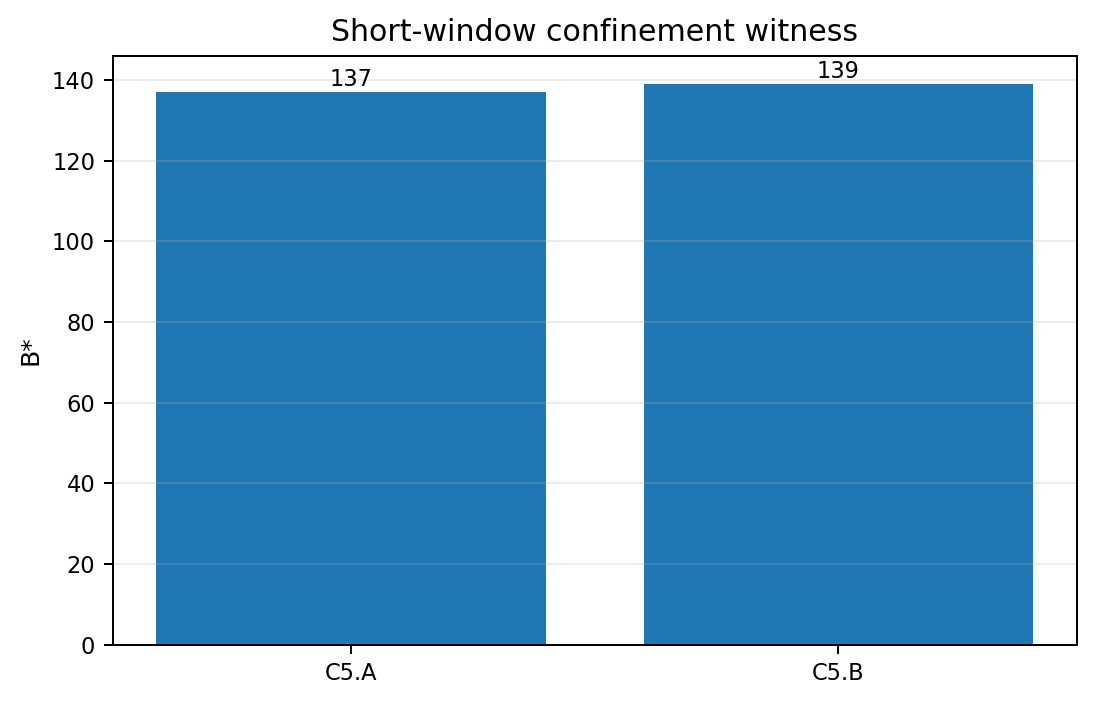
\includegraphics[width=0.72\linewidth]{figures/confinement/01_nucleus_confinement.png}
\caption{Short-window confinement witness.}
\label{fig:nucleus-confinement}
\end{figure}

The declared short row carries the proximity, confinement, and transmutation witnesses on one row.
